%& -shell-escape

%%% Copyright (c) 2010-2012, Илья w-495 Никитин
%%%
%%% Разрешается повторное распространение и использование
%%% как в виде исходного кода, так и в двоичной форме,
%%% если таковая будет получена, с изменениями или без,
%%% при соблюдении следующих условий:
%%%
%%% * При повторном распространении исходного кода
%%% должно оставаться указанное выше уведомление
%%% об авторском праве, этот список условий
%%% и последующий отказ от гарантий.
%%% * Ни имя w-495, ни имена друзей или консультантов
%%% не могут быть использованы в качестве поддержки
%%% или продвижения продуктов, основанных на этом коде
%%% без предварительного письменного разрешения.
%%%
%%% Этот код предоставлен владельцом авторских прав
%%% и/или другими сторонами <<как `она есть>>
%%% без какого-либо вида гарантий, выраженных явно
%%% или подразумеваемых, включая, но не ограничиваясь ими,
%%% (подразумеваемые) гарантии коммерческой ценности и пригодности
%%% для конкретной цели. Ни в коем случае, если не требуется
%%% соответствующим законом, или не установлено в устной форме,
%%% ни один владелец авторских прав и ни одно другое лицо,
%%% которое может изменять и/или повторно распространять программу,
%%% как было сказано выше, не несёт ответственности,
%%% включая любые общие, случайные, специальные
%%% или последовавшие убытки, вследствие использования
%%% или невозможности использования программы
%%% (включая, но не ограничиваясь потерей данных,
%%% или данными, ставшими неправильными, или потерями
%%% принесенными из-за вас или третьих лиц,
%%% или отказом программы работать совместно
%%% с другими программами), даже если такой владелец или другое
%%% лицо были извещены о возможности таких убытков.
%%%

%%% Документ нужно собирать только в XeLaTeX:
%%% $>xelatex имя-файла.tex
%%% Для этого должны быть установлены пакеты XeLaTeX и XeTeX
%%% в TeXLive или MikTeX или иной,
%%% если она поддерживает последние обновдения CTAN.

\documentclass[utf8,10pt,compress,hyperref={xetex}]{beamer}
\usepackage{styles/init}
\title[Статистический машинный перевод]
	{Распределенное программно-информационное обеспечение 
	статистической модели перевода естественных языков}  
\date{\today} 

\author{\today: И.\,К.~Никитин}

\begin{document}
	
	
\frame{
	\begin{center}
		{ \footnotesize \color{pacificgray} 
				МОСКОВСКИЙ АВИАЦИОННЫЙ ИНСТИТУТ \\
			(национальный исследовательский университет)
		} \\
		\vspace{35pt}
		{\Large 
			{\bfseries \color{pacificorange}
				Распределенное программно-информационное обеспечение
				статистической модели перевода естественных языков
			}
		}\\
		\vspace{35pt}
		\begin{tabular}{l}
			{ \color{pacificgray} 
				Выполнил студент группы 08-606} \\
			{
				\quad Никитин Илья Константинович} \\
					
			{ \color{pacificgray} 
				Научный руководитель }		\\ 
			{ \color{pacificgray} 
				ассистент кафедры 806}		\\
			{ 
				\quad Гаврилов Евгений Сергеевич}	\\
		\end{tabular} 
	\end{center}
} 


	
	\title[$\#\insertframenumber \le \inserttotalframenumber$~|~Статистический машинный перевод]{Распределенное программно-информационное обеспечение статистической модели перевода естественных языков}

	
\begin{frame}[t]
	\frametitle{Cодержание} 
	{
		\begin{multicols}{2}
			\tableofcontents 
		\end{multicols}
	}
\end{frame}




	\section{Введение} 

	
\subsection{Зачем}

\frame{
	\frametitle{Для чего нужен машинный перевод?} 
	\begin{itemize}
		\item бытовой перевод:
		\begin{itemize}	
			\item книги,
			\item переписка;
		\end{itemize} 
		\item поиск в Интернете на разных языках (внутри поисковых алгоритмов и дополнительная функция для пользователя);
		\item перевод научных публикаций c других языков;
		\item применения достижений в других областях:
		\begin{itemize}	
			\item автоматическое реферирование,
			\item распознавание речи,
			\item распознавание последовательностей аминокислот (ДНК).
		\end{itemize} 
	\end{itemize} 
}

	\subsection{Методы}
	
\frame{
	\frametitle{Основные методы машинного перевода} 
	\begin{center}
		\begin{scriptsize}
			\tikzstyle{rootf} = [draw=yellow!50!black!70,thick,minimum height=1cm,minimum width=2cm,top color=yellow!20,bottom color=yellow!60!black!20,decorate,decoration={random steps,segment length=3pt,amplitude=1pt}]
			\tikzstyle{basef-rule} = [rounded rectangle,thick,minimum size=1cm,draw=red!50!black!50,top color=white,bottom color=red!50!black!20,font=\itshape]
			\tikzstyle{typef-rule-i} = [rectangle,thick,minimum width=2cm,minimum height=1cm,draw=black!20,top color=white,bottom color=black!10]
			\tikzstyle{typef-rule-w} = [rectangle,thick,minimum width=2cm,minimum height=1cm,draw=orange!50!black!50,top color=white,bottom color=orange!50!black!20]
			\tikzstyle{typef-rule-t} = [rectangle,thick,minimum width=2cm,minimum height=1cm,draw=magenta!50!black!50,top color=white,bottom color=magenta!50!black!20]
			\tikzstyle{basef-data} = [rounded rectangle,thick,minimum size=1cm,draw=blue!50!black!50,top color=white,bottom color=blue!50!black!20]
			\tikzstyle{typef-data-e} = [rectangle,thick,minimum width=2cm,minimum height=1cm,draw=teal!50!black!50,top color=white,bottom color=teal!50!black!20]
			\tikzstyle{typef-data-s} = [rectangle,thick,minimum width=2cm,minimum height=1cm,draw=violet!50!black!50,top color=white,bottom color=violet!50!black!20]
			\tikzstyle{typef-mixed} = [rectangle,thick,minimum width=2cm,minimum height=1cm,draw=green!50!black!50,top color=white,bottom color=green!50!black!20]
			\begin{tikzpicture}[thick, node distance=2.5cm, text height=0.9ex, text depth=.25ex, auto]
				\node[rootf] (mt) {Машинный перевод};
				\node[basef-rule,below left of=mt] (rule) {Правила};
				\node[typef-rule-i,below right of=rule] (inter) {\color{black!40}Интерлингвистические};
				\node[typef-rule-w,below left of=rule] (words) {Пословные};		
				\node[typef-rule-t,below of=rule] (trans) {\bfseries Трансферные};
				\node[basef-data,below right of=mt] (data) {Данные};
				\node[typef-data-e,below right of=data] (ebmt) {Основанные на примерах};	
				\node[typef-data-s,below of=data] (smt) {\bfseries Статистические};
				%\node[typef-mixed,below left of=smt] (mixed) {\bfseries Смешанные};
				\path[->, red] (mt) edge (rule);		
				\path[->, red] (rule) edge (words);
				\path[->, red] (rule) edge (trans);
				\path[->, red!20] (rule) edge (inter);
				%\path[->, red] (trans) edge (mixed);
				\path[->, blue] (mt) edge (data);
				\path[->, blue] (data) edge (ebmt);	
				\path[->, blue] (data) edge (smt);	
				%\path[->, blue] (smt) edge (mixed);		
			\end{tikzpicture}
		\end{scriptsize}
	\end{center}
}




	

\section{Принципы} 

	
\subsection{Модель Шеннона}

\frame[allowframebreaks]{
	\frametitle{Модель зашумленного канала} 
	\def\drawnoisychanelpicture{
		\begin{center}
		\begin{scriptsize}
		\tikzstyle{rootf} = [draw=yellow!50!black!70,thick,minimum height=1cm,minimum width=2cm,top color=yellow!20,bottom color=yellow!60!black!20,decorate,decoration={random steps,segment length=3pt,amplitude=1pt}]
		\tikzstyle{pointf} = [rounded rectangle,thick,minimum size=1cm,draw=blue!50!black!50,top color=white,bottom color=blue!50!black!20]
		\tikzstyle{itemf} = [rectangle,thick,minimum width=2cm,minimum height=1cm,draw=teal!50!black!50,top color=white,bottom color=teal!50!black!20]
		\begin{tikzpicture}[thick, node distance=3cm, text height=0.9ex, text depth=.25ex, auto]
			\node[pointf] (source-point) {Передачик};
			\node[pointf,right of=source-point] (target-point) {Приемник};	
			\node[itemf,left of=source-point] (source) {Источник ($R$)};
			\node[itemf,right of=target-point] (target) {Цель ($E$)};	
				\path[->, black] (source) edge (source-point);
				\path [->, red, decoration={zigzag,segment length=5,amplitude=2,
					post=lineto,post length=2pt},font=\scriptsize,line join=round] 
						(source-point) edge[decorate] node[auto] {Шум} (target-point);
				\path[->, black] (target-point) edge (target);
		\end{tikzpicture}
		\end{scriptsize}
		\end{center}
	}
	
	\drawnoisychanelpicture
	
	\begin{small}
		\begin{enumerate}
			\item  Пусть $\FR$ --- фраза оригинала (русская).
			\item  Требуется найти $\FE$ --- фразу перевода (английскую).
			% \[
			%	\FE_g = \arg\max\limits_{\FE} P(\FE|\FR)
			% \]
		\end{enumerate}
		Максимизировать $P(\FE|\FR)$.
		\[
			P(\FE|\FR) =  \dfrac{\left( P(\FE) \cdot P(\FR|\FE) \right) }{P(\FR)}  \Rightarrow
		\]\[
			\FE_g = \arg\max\limits_{\cup \FE} P(\FE|\FR) =  \arg\max\limits_{\cup \FE} \left(  P(\FE) \cdot P(\FR|\FE) \right) 
		\]
		% $P(\FR)$ --- нам известна, ее не учитываем
	\end{small}
		% \pagebreak
		% 
		% \drawnoisychanelpicture 
		% 
		% \[
		% 	\arg\max\limits_{\cup \FE} P(\FE|\FR) =  \arg\max\limits_{\cup \FE} \left(  P(\FE) \cdot P(\FR|\FE) \right) 
		% \]
		% \begin{itemize}
		% 	\item  $\FR$ --- фраза оригинала (русская);
		% 	\item  $\FE$ --- фраза перевода (английская).
		% \end{itemize}	
}


{
	\tikzstyle{ssmpf} = [minimum height=1cm]
	\tikzstyle{lmf} = [circle,thick,minimum size=2.5cm,draw=blue!50!black!50,top color=white,bottom color=blue!50!black!20]
	\tikzstyle{tmf} = [circle,thick,minimum size=2.5cm,draw=green!50!black!50,top color=white,bottom color=green!50!black!20]
	\tikzstyle{dcf} = [circle,thick,minimum size=2.5cm,draw=red!50!black!50,top color=white,bottom color=red!50!black!20]
	\tikzstyle{corpf1} = [rectangle,rounded corners,thick,minimum size=2cm,draw=yellow!50!black!50,top color=white,bottom color=yellow!50!black!20]
	\tikzstyle{corpf2} = [rectangle,rounded corners,thick,minimum size=2cm,draw=yellow!50!black!50,top color=white,bottom color=yellow!50!black!20]
	\begin{frame}[t]
		\begin{center}
			\begin{scriptsize}
				\begin{tikzpicture}[thick, node distance=3.5cm, text height=0.2ex, text depth=.25ex, auto]
					\node[ssmpf] (ssmp) {Статистическая система машинного перевода};
					\node[lmf, below left of=ssmp] (lm) 
					{
						\begin{tabular}{c}
							Модель языка \\ 
							$ P(\FE) $\\ 
						\end{tabular} 
					};
					\node[tmf, below right of=ssmp] (tm)
					{
						\begin{tabular}{c}
							Модель перевода\\ 
							$ P(\FR|\FE) $\\ 
						\end{tabular} 
					};
					\path[->, black] (ssmp) edge (lm);
					\path[->, black] (ssmp) edge (tm);
				\end{tikzpicture}
			\end{scriptsize}
		\end{center}
		\[
			\arg\max\limits_{\cup \FE} P(\FE|\FR) =  \arg\max\limits_{\cup \FE} \left(  P(\FE) \cdot P(\FR|\FE) \right) 
		\]
		\begin{itemize}
			\item  $\FE$ --- фраза перевода (английская);
			\item  $\FR$ --- фраза оригинала (русская).
		\end{itemize}
	\end{frame}
	\begin{frame}[t]
		\begin{center}
			\begin{scriptsize}
				\begin{tikzpicture}[thick, node distance=3.5cm, text height=0.2ex, text depth=.25ex, auto]
					\node[ssmpf] (ssmp) {Статистическая система машинного перевода};
					\node[lmf, below left of=ssmp] (lm) 
					{
						\begin{tabular}{c}
							Модель языка \\ 
							$ P(\FE) $\\ 
						\end{tabular} 
					};
					\node[tmf, below right of=ssmp] (tm)
					{
						\begin{tabular}{c}
							Модель перевода\\ 
							$ P(\FR|\FE) $\\ 
						\end{tabular} 
					};
					\path[->, black] (ssmp) edge (lm);
					\path[->, black] (ssmp) edge (tm);		
					\node[dcf, below of=ssmp] (dc)
					{
							\begin{tabular}{c}
								{\large Декодер} \\ 
									\\
								% вычисляет \\
								$ \arg\max\limits_{\cup\FE} \left(  P(\FE) \cdot P(\FR|\FE) \right)$\\ 
							\end{tabular} 
					};	
					\path[->, black] (ssmp) edge (dc);
				\end{tikzpicture}
			\end{scriptsize}
		\end{center}
	\end{frame}
	\begin{frame}[t]
		\begin{center}
			\begin{scriptsize}
				\begin{tikzpicture}[thick, node distance=3.5cm, text height=0.2ex, text depth=.25ex, auto]
					\node[ssmpf] (ssmp) {Статистическая система машинного перевода};
					\node[lmf, below left of=ssmp] (lm) 
					{
						\begin{tabular}{c}
							Модель языка \\ 
							$ P(\FE) $\\ 
						\end{tabular} 
					};
					\node[corpf1, below of=lm] (lmr) 
					{
						\begin{tabular}{c}
							Корпус текста   \\ 
							на языке $\FE$. \\
						\end{tabular} 
					};
					\node[tmf, below right of=ssmp] (tm)
					{
						\begin{tabular}{c}
							Модель перевода\\ 
							$ P(\FR|\FE) $\\ 
						\end{tabular} 
					};
					\node[corpf2, below of=tm] (tmr) 
					{\tiny 
						\begin{tabular}{c}
							Параллельный \\
							корпус текста  \\ 
							на языках $\FE$ и $\FR$. \\ 
						\end{tabular} 
					};
					\path[->, black] (ssmp) edge (lm);
					\path[->, black] (ssmp) edge (tm);		
					\path[->, yellow!50!black!50] (lmr) edge (lm);
					\path[->, yellow!50!black!50] (tmr) edge (tm);		
					\node[dcf, below of=ssmp] (dc)
					{
							\begin{tabular}{c}
								{\large Декодер} \\ 
									\\
								% вычисляет \\
								$ \arg\max\limits_{\cup\FE} \left(  P(\FE) \cdot P(\FR|\FE) \right)$\\ 
							\end{tabular} 
					};	
					\path[->, black] (ssmp) edge (dc);
				\end{tikzpicture}
			\end{scriptsize}
		\end{center}
	\end{frame}
}


	
\subsection{Модель языка}

\frame{
	\frametitle{Модель языка}
	\small
	\begin{itemize}
		\item Правильный порядок слов.
		\item Вычисляется с помощью $n$-грамм слов. Пример для $3$-грамм:\\
		\[
			\FA = (\WA_1, \WA_2, \WA_3, \WA_4, \ldots, \WA_{\LA})
			\Rightarrow
			\left\lbrace 
				\begin{matrix}
					( \WA_1, &  \WA_2, &  \WA_3 );\\ 
					( \WA_2, &  \WA_3, &  \WA_4 );\\ 
					\vdots   &  \vdots &   \vdots \\ 	
					( \WA_{\LA-2}, &  \WA_{\LA-1}, &  \WA_{\LA} ).\\ 
				\end{matrix} 
			\right.
		\]
		\item Вычисляется по формуле:
		\[
			P(\FA)	= P( \WA_1 \ldots \WA_{\LA} ) = \prod\limits_{i=0}^{i=\LA+n-1} P'(\WA_i|\WA_{i-1} \ldots \WA_{i-n+1}).
		\]
	\end{itemize}
}

	

\subsection{Модель перевода}

\frame[allowframebreaks]{\frametitle{Модель перевода}
	\begin{itemize}
		\item Вводим выравнивание для пары предложений $\SE$, $\SR$.
		\item Для выравнивания нужны вероятности лексического перевода $\WE \rightarrow \WR$.
		\item Для вероятности лексического перевода нужны выравнивания.
		\item Проблема <<курицы и яйца>>.
	\end{itemize}
		
	\pagebreak
	
	Для оценки вероятности лексического перевода $\longrightarrow$ \\ EM-алгоритм (Витерби):
	\begin{itemize}
		\item инициализируем параметры модели (одинаковыми значениями, на первой итерации);
		\item оценим вероятности отсутствующей информации;
		\item оценим параметры модели на основании новой информации;
		\item перейдем к следующей итерации.
	\end{itemize}
}


	

\frame{
	\frametitle{\om Отличия от других систем} 
	% : отличия от других систем
	{\scriptsize 
		Система используется для перевода {\footnotesize \alert{научно-технической} литературы.}
		% Основываемся на стилистических особенностях научного текста.
	}\\
	\vspace{12pt}
	\greenbox{Слова $\rightarrow$ $n$-грамы }
	{\footnotesize
		\begin{itemize}
			\item[$\Leftarrow$] Устойчивые формальные выражения в научных текстах.
		\end{itemize}
	}
	\vspace{12pt}
	\bluebox{Выравнивание по круппным группам $n$-грам}
	{\footnotesize
		\begin{itemize}
			\item[$\Leftarrow$] прямой порядок слов;
			\item[$\Leftarrow$] стереотипная структура предложений.
		\end{itemize}
	}
	\vspace{12pt}
	\orangebox{Модели низких порядков}
	{\footnotesize
		\begin{itemize}
			\item[$\Leftarrow$] важность локального порядка слов;
			\item[$\Leftarrow$] фертильности и вероятностной грамматики могут его разрушить.
		\end{itemize}
	
	}
}



	
\subsection{Декодер}

\frame{
	\frametitle{Декодер}
	\small
	\begin{columns}
		\begin{column}{6cm}
			Среди всех возможных вариантов перевода выбрать правильный:
			\begin{itemize}
				\item полный перебор;
				\item A*:
				\begin{itemize}
					\item стековый поиск,
					\item многостековый поиск;
				\end{itemize}
				\item \textbf{жадный инкрементный поиск};
				\item сведение к обобщенной задаче коммивояжера.
					% \begin{itemize}
					%	\item задача ЛП,
					%	\item эвристические методы (Лин-Керниган),
					%	\item генетические алгоритмы,
					%	\item {<<муравьиная оптимизация>>}.
					% \end{itemize}
			\end{itemize}
		\end{column}
		\begin{column}{4cm}
			\tikzstyle{ssmpf} = [minimum height=1cm]
			\tikzstyle{lmf} = [circle,thick,minimum size=1.5cm,draw=blue!50!black!50,top color=white,bottom color=blue!50!black!20]
			\tikzstyle{tmf} = [circle,thick,minimum size=1.5cm,draw=green!50!black!50,top color=white,bottom color=green!50!black!20]
			\tikzstyle{dcf} = [circle,thick,minimum size=1.5cm,draw=red!50!black!50,top color=white,bottom color=red!50!black!20]
			\begin{tiny}
				\begin{tikzpicture}[thick, node distance=1.9cm, text height=0.2ex, text depth=.25ex, auto]
					\node(ssmp) {};
					\node[lmf, below right of=ssmp] (lm) 
					{\begin{tabular}{c}
						Модель \\ языка \\  $ P(\FE) $\\ 
					\end{tabular}};
					\node[tmf, below left of=ssmp] (tm)
					{\begin{tabular}{c}
						Модель \\ перевода\\ $ P(\FR|\FE) $\\ 
					\end{tabular} };
					\node[dcf, below of=ssmp] (dc) {\small Декодер};	
					\begin{scope}[node distance=2.0cm]
						\node[ssmpf, above of=dc] (source)
						{ \scriptsize
							\begin{tabular}{c}
								Исходная фраза \\ $ \FR $\\ 
							\end{tabular} 
						};
						\node[ssmpf, below of=dc] (target)
						{ \scriptsize
							\begin{tabular}{c}
								Перевод исходной фразы \\
								$ \arg\max\limits_{\FE} \left(  P(\FE) \cdot P(\FR|\FE) \right)$\\ 
							\end{tabular} 
						};
					\end{scope}
					\path[->, gray] (source) edge (dc);
					\path[->, gray] (dc) edge (target);
				\end{tikzpicture}
			\end{tiny}
		\end{column}
	\end{columns}
}

\frame{
	\frametitle{Жадный инкрементный поиск} 
	\begin{itemize}
		\item простой и быстрый поиск;
		\item {<<плохой>> вариант перевода получаем сразу};
		\item последовательно применяя набор операций можем улучшить перевод;
		\begin{itemize}	
			\item изменить перевод слова \textit{(группы слов, $n$-граммы)},
			\item удалить слово \textit{(группу слов, $n$-грамму)},
			\item поменять слова местами \textit{(группы слов, $n$-граммы)};
		\end{itemize} 
		\item можно делать отсечку по времени;
		\item можем сразу оценить модель языка большой фразы.
	\end{itemize} 
}








	\section{Архитектура} 

	
\subsection{Обзор}

\frame{
	\frametitle{\om Из чего состоит система} 
		\tikzstyle{databasef} = [rectangle,thick,minimum size=1cm,draw=teal!50!black!50,top color=white,bottom color=teal!50!black!20,font=\itshape]
		\tikzstyle{readerf} = [rectangle,rounded corners,thick,minimum size=1cm,draw=blue!50!black!50,top color=white,bottom color=blue!50!black!20,font=\itshape]
		\tikzstyle{handlerf} = [rectangle,rounded corners,thick,minimum size=1cm,draw=green!50!black!50,top color=white,bottom color=green!50!black!20,font=\itshape]
		\tikzstyle{decoderf} = [rounded rectangle,thick,minimum size=1cm,draw=red!50!black!50,top color=white,bottom color=red!50!black!20,font=\itshape]
		\tikzstyle{humanf} = [rounded rectangle,thick,minimum size=1.2cm]
		\tikzstyle{decoderif} = [rounded rectangle,thick,minimum size=0.5cm,draw=red!50!black!50,top color=white,bottom color=red!50!black!20,font=\itshape]
		\tikzstyle{corporaf} = [draw=yellow!50!black!70,thick,minimum height=1cm,minimum width=1cm,top color=yellow!20,bottom color=yellow!60!black!20,decorate,decoration={random steps,segment length=3pt,amplitude=1pt}]
	\begin{tikzpicture}[thick, node distance=3cm, text height=1.5ex, text depth=.25ex, auto]
		\node[databasef] 						(database)	{
			\footnotesize 
			\begin{tabular}{c}
				{\small База данных} \\
				{$\vartriangleright$} Redis
			\end{tabular} 
		};
		\begin{scope}[node distance=2.5cm]
			\node[above right of=database]	(name)	{
				\Large \Malgun ПРС-СМП
			};
		\end{scope}
		\begin{scope}[node distance=4cm]
			\node[left of=database] 	(comment)	{
				\scriptsize
				\begin{tabular}{l}
					{\color{pacificorange} $\blacktriangleright$} Набор приложений.\\
					{\color{pacificorange} $\blacktriangleright$} Могут быть удалены\\
						\qquad друг от друга.\\
					{\color{pacificorange} $\blacktriangleright$} Распределены\\
						\qquad где это возможно.\\
				\end{tabular} 
			};
		\end{scope}
		\node[readerf,above left of=database]	(reader)	{
			\footnotesize 
			\begin{tabular}{c}
				{\small Читатель} \\
				{$\vartriangleright$} Erlang
			\end{tabular} 
		};
		\node[corporaf,left of=reader]			(corpora)	{\small Корпус En, Ru};
		\node[handlerf,below left of=database]	(handler)	{
			\footnotesize 
			\begin{tabular}{c}
				{ \small Обработчик }\\
				{$\vartriangleright$} Erlang
			\end{tabular} 
		};
		\node[decoderf,right of=database]		(decoder)	{
			\footnotesize 
			\begin{tabular}{c}
				{ \small Декодер } \\
				{$\vartriangleright$} Erlang
			\end{tabular} 
		};
		\begin{scope}[node distance=1.9cm]		
			\node[decoderif,below left  of=decoder]		(decoderweb)	{\footnotesize Веб};
			\node[decoderif,below 	   of=decoder]		(decodercon)	{\footnotesize Консоль};
			\node[decoderif,below right of=decoder]		(decoderrest)	{\footnotesize Rest};
		\end{scope}
		
		\begin{scope}[node distance=1.2cm]		
			\node[humanf,		below 	   of=decodercon]		(human)	{
				\begin{tabular}{c}
					
\includegraphics[height=1.2cm]{./vec/arch-human.eps} \\
				\end{tabular} 
			};
		\end{scope}
		\path[->, yellow!40!black!70] 	(corpora)	edge (reader);
		\path[<-, blue] 				(database)	edge (reader);
		\path[<->, blue] 				(database)	edge (handler);
		\path[<->, red] 				(database)	edge (decoder);
		\path[-, red, dotted] 			(decoder)	edge node[auto] {\scriptsize интерфейсы} (decoderweb);
		\path[-, red, dotted] 			(decoder)	edge (decodercon);
		\path[-, red, dotted] 			(decoder)	edge (decoderrest);
		\path[<->, red] 				(human)	edge (decoderweb);
		\path[<->, red] 				(human)	edge (decodercon);
		\path[<->, red] 				(human)	edge (decoderrest);
	\end{tikzpicture}
}


	\subsection{Обучение}

\begin{frame}[t] % [plain]
	\begin{columns}
		\begin{column}{2.7cm}
			\graybox{Читатель}{
				\begin{center}
					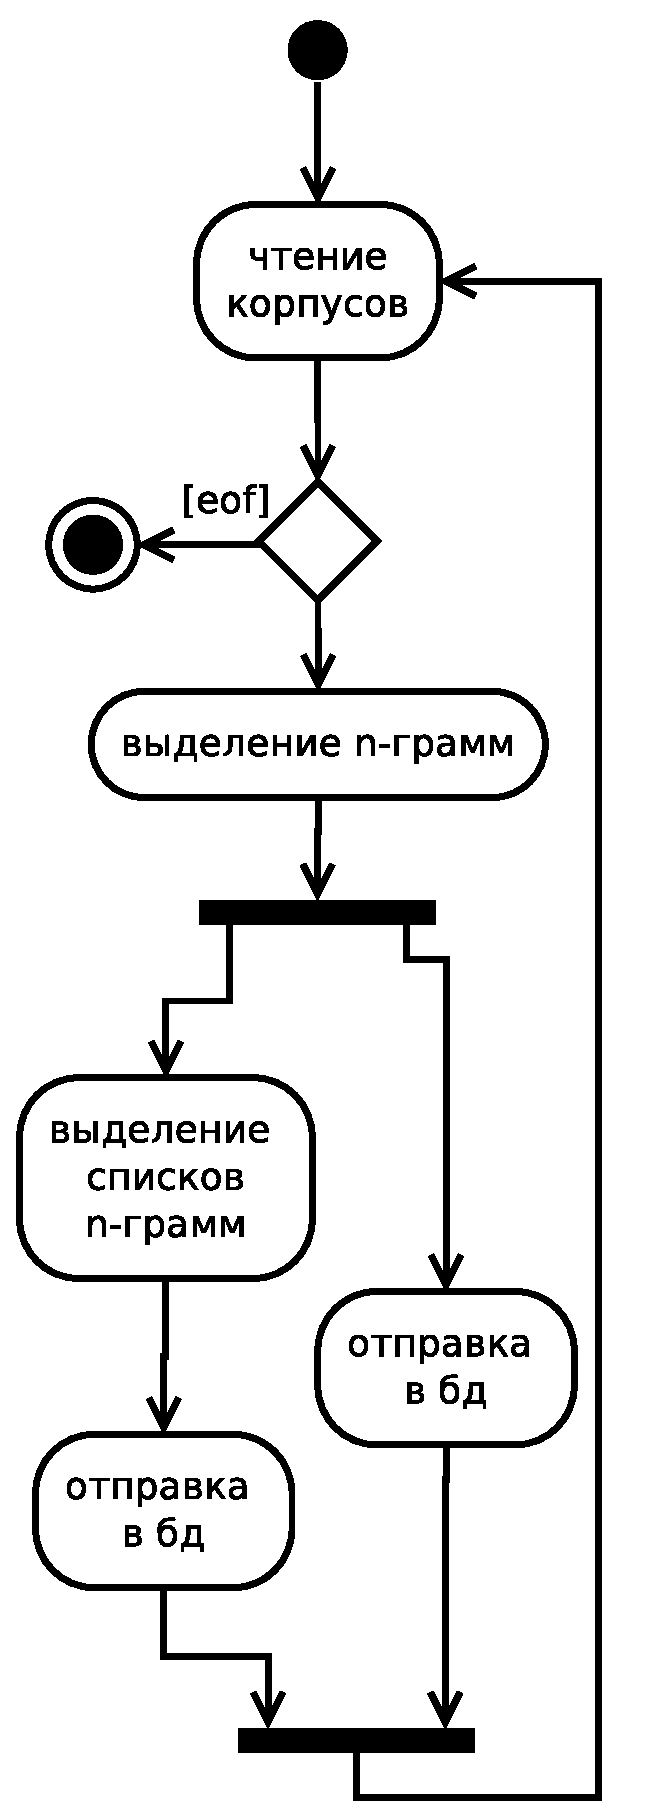
\includegraphics[height=7.5cm]{./vec/arch-reader.eps}
				\end{center}
			}
		\end{column}
		\begin{column}{2cm}
			\begin{scriptsize}
				\[
					N_{\text{чит.}} < N_{\text{обр.}}
				\]
			\end{scriptsize}
		\end{column}
		\begin{column}{5.2cm}
			\graybox{Обработчик}{
				\begin{center}
					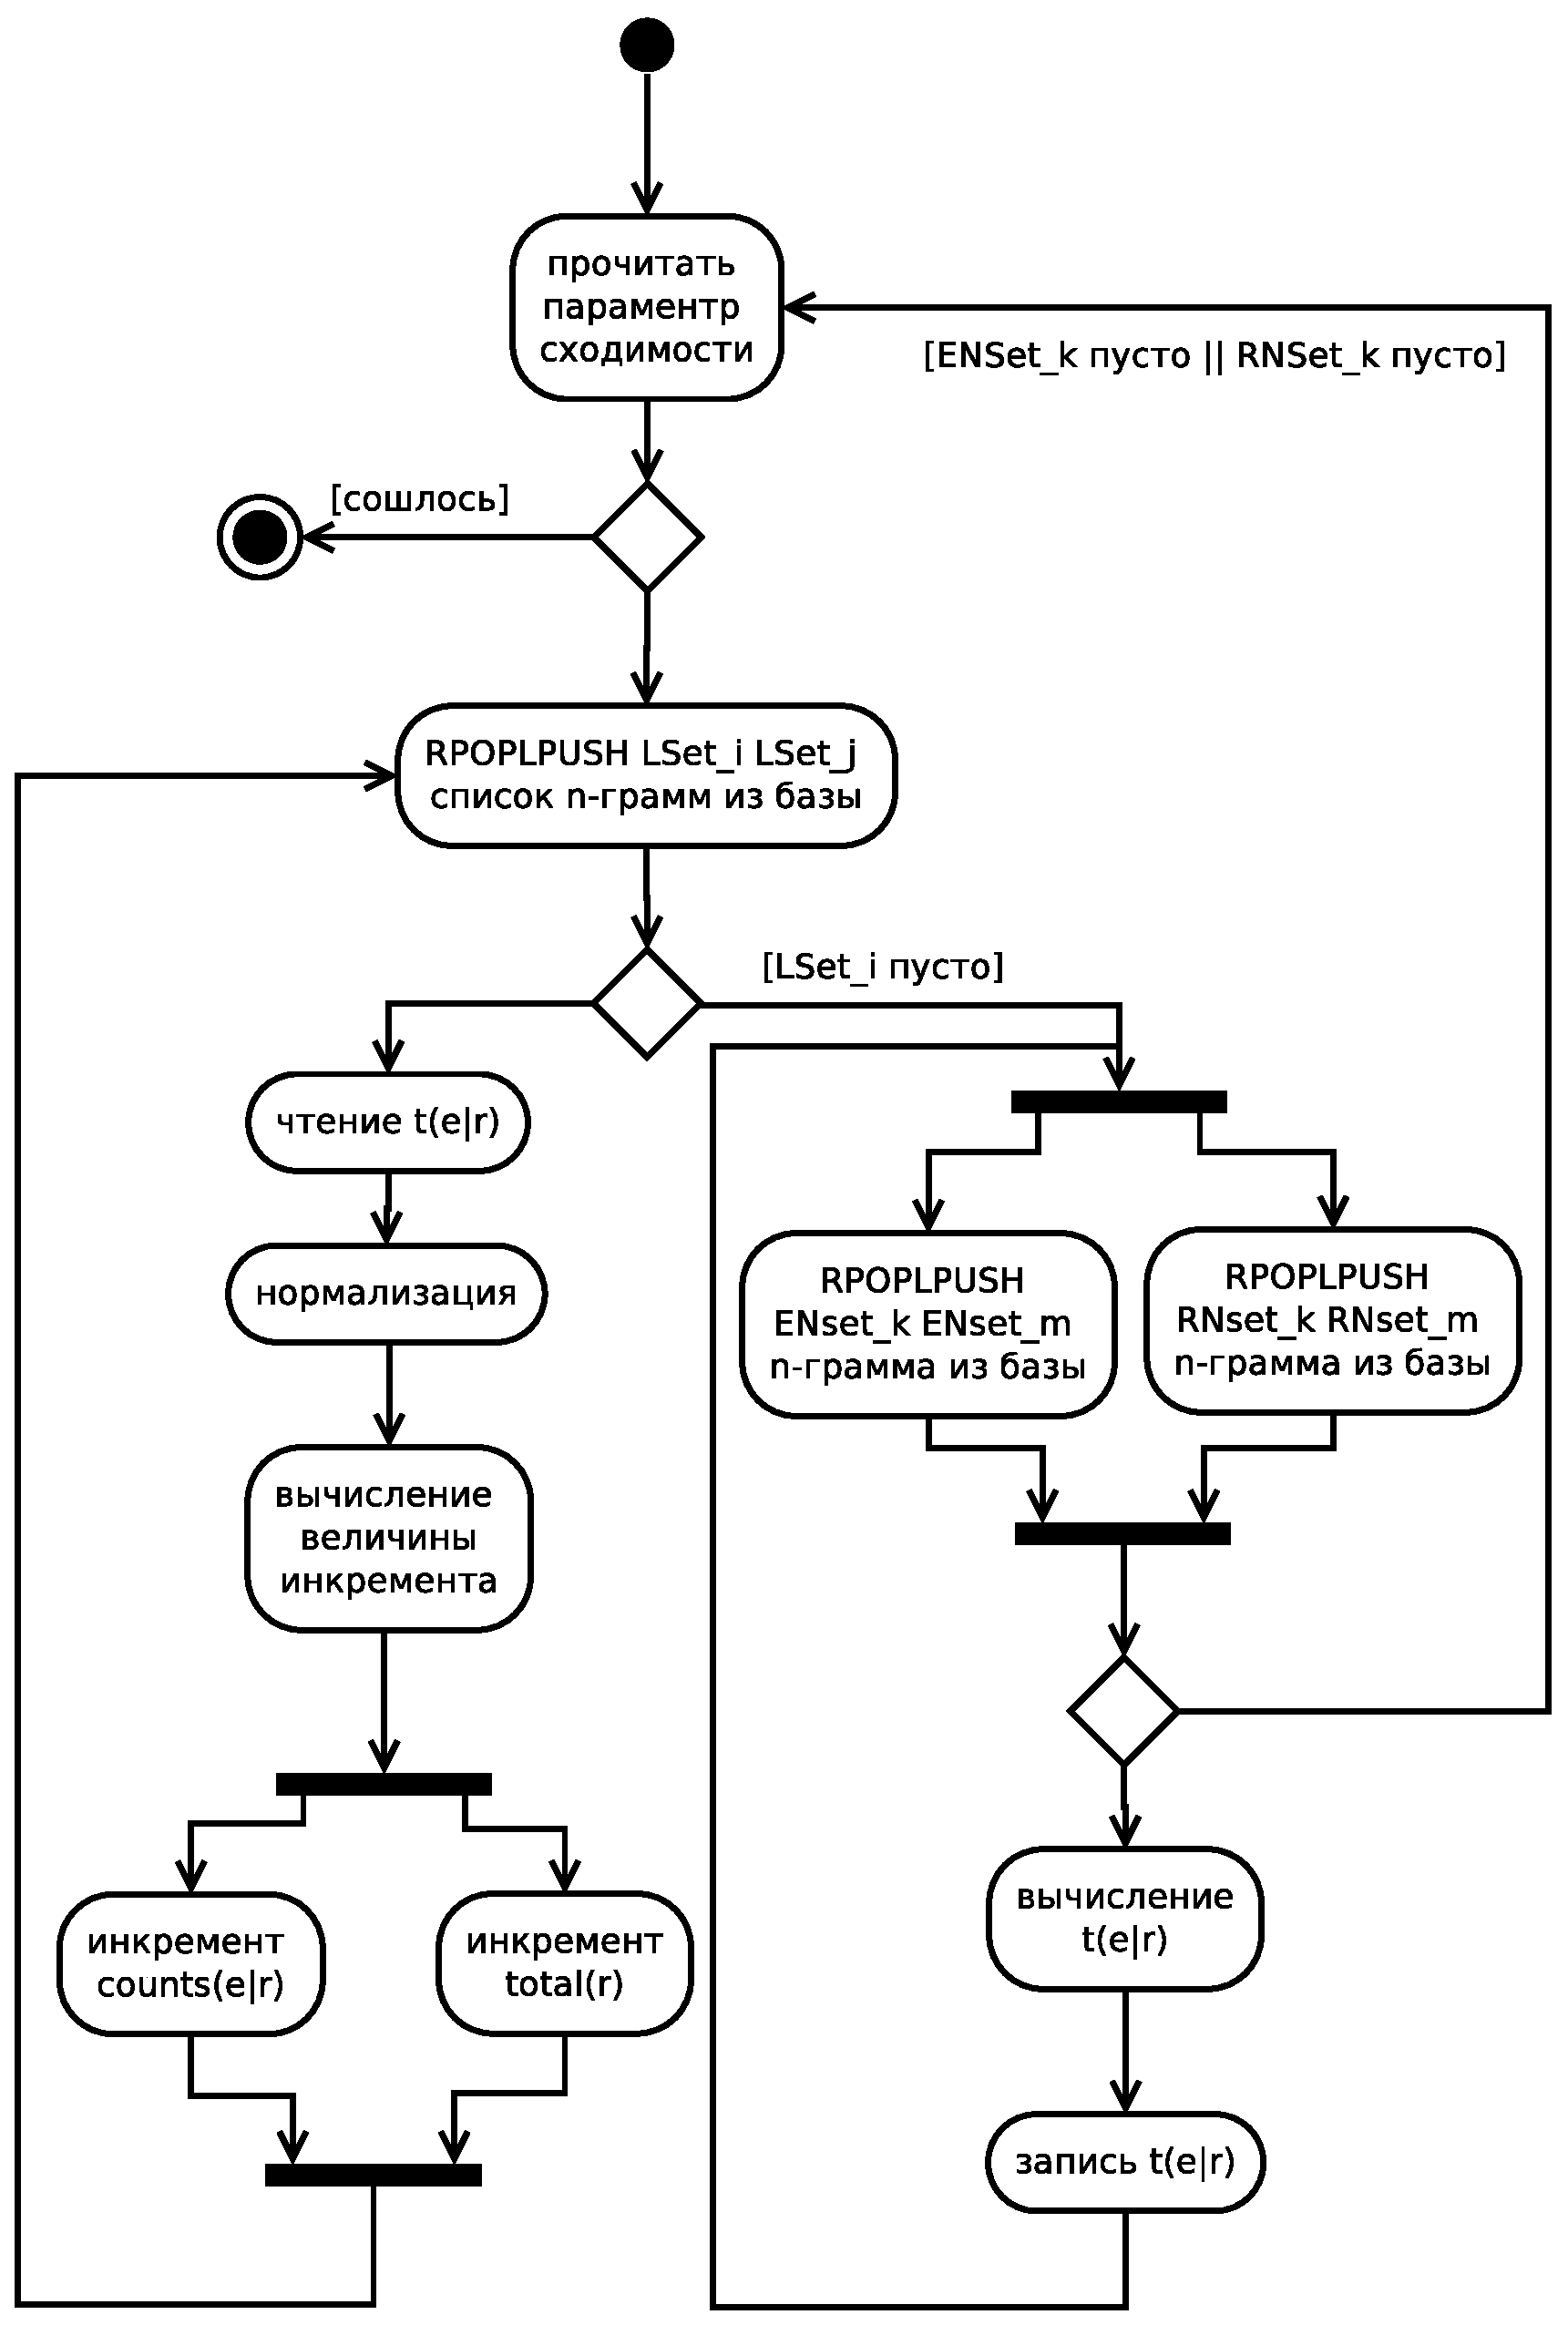
\includegraphics[height=7.5cm]{./vec/arch-handler.eps}
				\end{center}
			}
		\end{column}
	\end{columns}
\end{frame}

	
\subsection{Декодеривание}

\begin{frame}[t] % [plain]
	\begin{columns}
		\begin{column}{6.5cm}
			\graybox{Декодер}{
				\begin{center}
					\includegraphics[height=7.5cm]{./vec/arch-decoder.eps}
				\end{center}
			}
		\end{column}
		\begin{column}{5cm}
			\small
			\begin{itemize}
				\item жадный инкрементный поиск;
				\item два режима работы:
				\begin{itemize}
					\item перевода,
					\item улучшения.
				\end{itemize}
				\item пошаговый веб-интерфейс;
				\item потоковый RESTful-сервис;
				\item пошаговый консольный интерфейс.
			\end{itemize}
		\end{column}
	\end{columns}
\end{frame}

	



	\addtocontents{toc}{\protect\pagebreak} 
	

\section{Оценка}

	\subsection{Примеры}

\frame[allowframebreaks]{
	\frametitle{\om Примеры}
	% =================================
	\begin{block}{Оригинал}
		... adopted at~the 81st plenary meeting ...
	\end{block}
	\begin{exampleblock}{Переводчик}
		... принята на~81-м пленарном заседании ...
	\end{exampleblock}
	\begin{alertblock}{Система}
		... принята без~голосования на~81 пленарном заседании в~Брюсселе ...
	\end{alertblock}
	% =================================
	\pagebreak
	\begin{block}{Оригинал}
		It will be instructive to exhibit Euclid's algorithm here.
	\end{block}
	\begin{exampleblock}{Переводчик}
		Думаю, имеет смысл привести здесь описание этого алгоритма.
	\end{exampleblock}
	\begin{alertblock}{Система}
		Будет поучительно выставить алгоритм Евклида здесь.
	\end{alertblock}
	% =================================
	\pagebreak
	\begin{block}{Оригинал}
		Many years have passed since the author wrote most of the comments above ...
	\end{block}
	\begin{exampleblock}{Переводчик}
		Со времени первого написания автором большинства приведенных выше комментариев \underline{утекло много воды} ...
	\end{exampleblock}
	\begin{alertblock}{Система}
		Много лет прошло с тех пор\underline{,} автор написал большую часть комментариев выше ...
	\end{alertblock}
}


	
\subsection{BLEU}

\frame{
	\frametitle{Оценка перевода с использованием метрики BLEU}
	\begin{columns}
			\begin{column}{7cm}
				\small
				\begin{itemize}
					\item BLEU --- Bilingual Evaluation Understudy
					\item Численная оценка качества перевода.
					\item Нужен перевод, выполненный человеком.
					\item Показывает величину близости 
						к~<<человеческому>> переводу.
					\item Чем меньше величина, тем лучше.
					\item Сравнивались:
						\begin{itemize}
							\item ПРС-СМП;
							\item cистемы построенная на~основе Moses.
						\end{itemize}
				\end{itemize}
			\end{column}
			\begin{column}{5cm}
					\begin{tabular}{|r|r|}
						\hline  \textbf{Система}	&	\textbf{BLEU}  \\ 
						\hline  ПРС-СМП (1)			&	0.243 \\ 
						\hline  ПРС-СМП (100)		&	0.209 \\ 
						\hline  Moses (IBM 3)		&	0.201 \\ 
						\hline  Moses (IBM 5) 		& 	0.173 \\ 
						\hline 
					\end{tabular} 
			\end{column}
		\end{columns}
}

	\subsection{Скорость}

\frame{
	\frametitle{Оценка скорости обучения}
	Процессор: Intel Core2 Duo, 1 ядро 64 бит, ОП 4Гб, ФС:ext4
	\begin{center}
	    \begin{tabular}{|r|r|}
	        \hline  \textbf{Система}        & \textbf{Время, ч} \\
	        \hline  ПРС-СМП (1)             &   $ \approx $ 5   \\
	        \hline  Moses (GIZA++)          &   $ \approx $ 25  \\
	        \hline  Chaski (MGIZA++)        &   $ \approx $ 26  \\
	        \hline
	    \end{tabular}
	\end{center}
	Процессор: Intel Xeon E5506, 8 ядер 64 бит, ОП 10Гб, ФС:xfs
	\begin{center}
	    \begin{tabular}{|r|r|}
	        \hline  \textbf{Система}    & \textbf{Время, ч} \\
	        \hline  ПРС-СМП (1)         &   $ \approx $ 1   \\
	        \hline  Moses (GIZA++)      &   $ \approx $ 22  \\
	        \hline  Chaski (MGIZA++)    &   $ \approx $ 3   \\
	        \hline
	    \end{tabular}
	\end{center}
}

\frame{
	\frametitle{Оценка скорости декодирования}
	Процессор: Intel Core2 Duo, 1 ядро 64 бит, ОП 4Гб, ФС:ext4
	\begin{center}
	    \begin{tabular}{|r|r|}
	        \hline  \textbf{Система}    &   \textbf{Время, мкс} \\
	        \hline  ПРС-СМП (1)         &   1132 \\
	        \hline  ПРС-СМП (100)       &   7108124  \\
	        \hline  Moses (IBM 3)       &   $\approx$ 10000000\\
	        \hline  Moses (IBM 5)       &   $\approx$ 30000000 \\
	        \hline
	    \end{tabular}
	\end{center}
	Процессор: Intel Xeon E5506, 8 ядер 64 бит, ОП 10Гб, ФС:xfs
	\begin{center}
	    \begin{tabular}{|r|r|}
	        \hline  \textbf{Система}    &   \textbf{Время, мкс} \\
	        \hline  ПРС-СМП (1)         &   1012 \\
	        \hline  ПРС-СМП (100)       &   1119024  \\
	        \hline  Moses (IBM 3)       &   $\approx$ 5000000\\
	        \hline  Moses (IBM 5)       &   $\approx$ 6000000 \\
	        \hline
	    \end{tabular}
	\end{center}
}



	%
\subsection{Цена}

\frame{
	\frametitle{Оценка полезности}
	\begin{columns}
		\begin{column}[t]{6cm}
			\textbf{Экономическая часть:}
			\begin{itemize}
				\item Разработка --- $916669$ руб.
				\item Цена --- $1833$ руб.
				\item Стоимость --- $108786$ руб/год.
				\item Меньше зп плохого переводчика ($385920$ руб/год).
			\end{itemize}
		\end{column}
		\begin{column}[t]{6cm}
			\textbf{Охрана труда:}
			\begin{itemize}
				\item Хороший переводчик меньше проводит время у компьютера.
				\item Не подвергается вредному воздействию:
				\begin{itemize}
					\item \textbf{тихо} работает $\Rightarrow$;
					\item  $\Rightarrow$ качественный перевод $\Rightarrow$;
					\item  $\Rightarrow$ качественные данные.
				\end{itemize}
			\end{itemize}
		\end{column}
	\end{columns}
}




	\section{Перспективы}

	\subsection{Результаты}

\frame{
	\frametitle{Результаты} 
	\begin{itemize}
		\item \alert{Разработан} подход:
		\begin{itemize}
			\item быстрого обучения модели перевода для научных текстов.
		\end{itemize}
		\item \alert{Реализована} система машинного перевода:
		\begin{itemize}
			\item многопроцессорная, распределенная;
			\item только научно-техническая литература;
			\item быстрое обучение;
			\item быстрое (пошаговое) декодирование.
		\end{itemize}
	\end{itemize}
}


	
\subsection{Развитие} 

\frame{
	\frametitle{Дальнейшее развитие} 
	\begin{columns}
		\begin{column}[t]{6cm}
			\small
			\textbf{Математика:}
			\begin{itemize}
				\item полноценный фразовый перевод;
				\item синтаксический перевод;
				\item смешанная система перевода:
				\begin{itemize}
					\item пара русский-английский,
					\item морфологический анализ.
				\end{itemize}
				\item опробовать более точные методы поиска.
			\end{itemize}
		\end{column}
		\begin{column}[t]{6cm}
			\small
			\textbf{Архитектура и реализация:}
			\begin{itemize}
				\item использовать пословное сжатие при хранении в БД;
				\item переписать обработчика на Cи с libevent;
				\item libevent для RESTful-сервиса декодера:
				\begin{itemize}
					\item 1 млн. одновременных соединений
				\end{itemize}
				\item попробовать Redis $\rightarrow$ leveldb.
			\end{itemize}
		\end{column}
	\end{columns}
}



	\subsection{Результаты}

\frame{
	\frametitle{Результаты} 
	\begin{itemize}
		\item \alert{Разработан} подход:
		\begin{itemize}
			\item быстрого обучения модели перевода для научных текстов.
		\end{itemize}
		\item \alert{Реализована} система машинного перевода:
		\begin{itemize}
			\item многопроцессорная, распределенная;
			\item только научно-техническая литература;
			\item быстрое обучение;
			\item быстрое (пошаговое) декодирование.
		\end{itemize}
	\end{itemize}
}


		


	
\section{+} 

	
\frame{
	\begin{center}
		\vspace{45pt}
		{\Large \bfseries \color{pacificorange}
			Приложения-подробности
		}\\
		{\color{pacificgray}
			интересные слайды,\\
			которые не вошли в саму презентацию
		}\\
		\vspace{55pt}
	\end{center}
} 


	
\subsection{Модель языка}

\frame{
	\frametitle{Модель языка}
	\small
	\begin{itemize}
		\item Правильный порядок слов.
		\item Вычисляется с помощью $n$-грамм слов. Пример для $3$-грамм:\\
		\[
			\FA = (\WA_1, \WA_2, \WA_3, \WA_4, \ldots, \WA_{\LA})
			\Rightarrow
			\left\lbrace 
				\begin{matrix}
					( \WA_1, &  \WA_2, &  \WA_3 );\\ 
					( \WA_2, &  \WA_3, &  \WA_4 );\\ 
					\vdots   &  \vdots &   \vdots \\ 	
					( \WA_{\LA-2}, &  \WA_{\LA-1}, &  \WA_{\LA} ).\\ 
				\end{matrix} 
			\right.
		\]
		\item Вычисляется по формуле:
		\[
			P(\FA)	= P( \WA_1 \ldots \WA_{\LA} ) = \prod\limits_{i=0}^{i=\LA+n-1} P'(\WA_i|\WA_{i-1} \ldots \WA_{i-n+1}).
		\]
	\end{itemize}
}

	

\subsection{Модель перевода}

\frame[allowframebreaks]{\frametitle{Модель перевода}
	\begin{itemize}
		\item Вводим выравнивание для пары предложений $\SE$, $\SR$.
		\item Для выравнивания нужны вероятности лексического перевода $\WE \rightarrow \WR$.
		\item Для вероятности лексического перевода нужны выравнивания.
		\item Проблема <<курицы и яйца>>.
	\end{itemize}
		
	\pagebreak
	
	Для оценки вероятности лексического перевода $\longrightarrow$ \\ EM-алгоритм (Витерби):
	\begin{itemize}
		\item инициализируем параметры модели (одинаковыми значениями, на первой итерации);
		\item оценим вероятности отсутствующей информации;
		\item оценим параметры модели на основании новой информации;
		\item перейдем к следующей итерации.
	\end{itemize}
}


	
\subsection{Декодер}

\frame{
	\frametitle{Декодер}
	\small
	\begin{columns}
		\begin{column}{6cm}
			Среди всех возможных вариантов перевода выбрать правильный:
			\begin{itemize}
				\item полный перебор;
				\item A*:
				\begin{itemize}
					\item стековый поиск,
					\item многостековый поиск;
				\end{itemize}
				\item \textbf{жадный инкрементный поиск};
				\item сведение к обобщенной задаче коммивояжера.
					% \begin{itemize}
					%	\item задача ЛП,
					%	\item эвристические методы (Лин-Керниган),
					%	\item генетические алгоритмы,
					%	\item {<<муравьиная оптимизация>>}.
					% \end{itemize}
			\end{itemize}
		\end{column}
		\begin{column}{4cm}
			\tikzstyle{ssmpf} = [minimum height=1cm]
			\tikzstyle{lmf} = [circle,thick,minimum size=1.5cm,draw=blue!50!black!50,top color=white,bottom color=blue!50!black!20]
			\tikzstyle{tmf} = [circle,thick,minimum size=1.5cm,draw=green!50!black!50,top color=white,bottom color=green!50!black!20]
			\tikzstyle{dcf} = [circle,thick,minimum size=1.5cm,draw=red!50!black!50,top color=white,bottom color=red!50!black!20]
			\begin{tiny}
				\begin{tikzpicture}[thick, node distance=1.9cm, text height=0.2ex, text depth=.25ex, auto]
					\node(ssmp) {};
					\node[lmf, below right of=ssmp] (lm) 
					{\begin{tabular}{c}
						Модель \\ языка \\  $ P(\FE) $\\ 
					\end{tabular}};
					\node[tmf, below left of=ssmp] (tm)
					{\begin{tabular}{c}
						Модель \\ перевода\\ $ P(\FR|\FE) $\\ 
					\end{tabular} };
					\node[dcf, below of=ssmp] (dc) {\small Декодер};	
					\begin{scope}[node distance=2.0cm]
						\node[ssmpf, above of=dc] (source)
						{ \scriptsize
							\begin{tabular}{c}
								Исходная фраза \\ $ \FR $\\ 
							\end{tabular} 
						};
						\node[ssmpf, below of=dc] (target)
						{ \scriptsize
							\begin{tabular}{c}
								Перевод исходной фразы \\
								$ \arg\max\limits_{\FE} \left(  P(\FE) \cdot P(\FR|\FE) \right)$\\ 
							\end{tabular} 
						};
					\end{scope}
					\path[->, gray] (source) edge (dc);
					\path[->, gray] (dc) edge (target);
				\end{tikzpicture}
			\end{tiny}
		\end{column}
	\end{columns}
}

\frame{
	\frametitle{Жадный инкрементный поиск} 
	\begin{itemize}
		\item простой и быстрый поиск;
		\item {<<плохой>> вариант перевода получаем сразу};
		\item последовательно применяя набор операций можем улучшить перевод;
		\begin{itemize}	
			\item изменить перевод слова \textit{(группы слов, $n$-граммы)},
			\item удалить слово \textit{(группу слов, $n$-грамму)},
			\item поменять слова местами \textit{(группы слов, $n$-граммы)};
		\end{itemize} 
		\item можно делать отсечку по времени;
		\item можем сразу оценить модель языка большой фразы.
	\end{itemize} 
}



	
\subsection{BLEU}

\frame{\frametitle{BLEU --- Bilingual Evaluation Understudy}
	{\small
	\[
	    \mathrm{BLEU} = Bp \cdot e^{ \left(  \sum\limits_{n=1}^{N} W_n \log(p_n) \right) }
	\]\[
	    Bp = \left\lbrace
	        \begin{array}{cc}
	            1, &  l_c > l_h;\\
	            e^{\left(1 - \frac{l_h}{l_c}\right)}, &  l_c \le l_h.\\
	        \end{array}
	    \right.
	    \quad \text{ и }\quad
	    p_n =
	        \dfrac{\sum\limits_{C \in S_c}  \sum\limits_{\eta_c \in C} \text{\it число}_{\text{среза}}(\eta_c) }
	            {\sum\limits_{C \in S_c}  \sum\limits_{\eta_c \in C} \text{\it число}(\eta_c) }
	\]
	}
	\begin{columns}
			\begin{column}{6cm}
				\scriptsize
				\begin{itemize}
					\item $S_c$ --- множество кандидатов на перевод;
					\item $C$ --- кандидат на перевод; 
					\item $\eta_c$ --- $n$-грамма кандидата на перевод;
					\item $l_c$ --- длинна кандидата перевода;
					\item $l_h$ --- длинна экспертного перевода (выполненного человеком);
					\item $W_n = \dfrac{1}{N}$ --- вес;
					\item $N = 4$, $n$-граммность оценки.
				\end{itemize}
			\end{column}
			\begin{column}{5cm}
				\small
					\begin{tabular}{|r|r|}
						\hline  \textbf{Система}	&	\textbf{BLEU}  \\ 
						\hline  ПРС-СМП (1)			&	0.243 \\ 
						\hline  ПРС-СМП (100)		&	0.209 \\ 
						\hline  Moses (IBM 3)		&	0.201 \\ 
						\hline  Moses (IBM 5) 		& 	0.173 \\ 
						\hline 
					\end{tabular} 
			\end{column}
		\end{columns}
}



\end{document}


